The problem of attesting to one's location is a fundamental act of metaphysical reasoning that happens everywhere, at every moment. Unconsciously and unwittingly, we do claim to be somewhere at an indiscriminated point in time, and we do expect others to believe in us. However, this act is grounded on informal and implicit levels of trust that are not often explicitly asserted, as liability is usually not categorically assigned. When it does happen, trust is usually delegated to a third party or distributed between multiple parties, that may be able to testify to one's presence, synchronously, at the very same location. The act of witnessing is, therefore, a regular yet fundamental part of our interactions with physical reality. When we do claim our presence at an event, assert our location to a service provider, or even state our alibi to authorities, as defense in a criminal charge, a protocol for location attestation is implicitly followed. Some may require a physical interaction of any kind, while others may find digitalized and infrastructural means to gather the required location proof \cite{luo2010veriplace}.

A digital \pol{} can then be defined as an electronic certificate that assuredly attests one's relative position in both space and time \cite{amoretti2018blockchain}. The relativity of the attestation is, nevertheless, a non-trivial matter. It is, in fact, a complex and multi-faceted process that requires the simultaneous existence of various untrusted or semi-trusted parties, especially in an environment with no individual honesty guarantees. According to Nasrulin et al. \cite{nasrulin2018robust}, a \pol{} protocol may be considered secure if complete, spatio-temporally sound, and non-transferable. Consequently, the system that materially backs the implementation of such a protocol is expected to provide fault-tolerance, reliability, and availability guarantees. More advanced protocols may also explore the possibility of providing privacy and anonymity assurances \cite{li2020privacy}, as well as the possibility of being used in a fully trustless environment \cite{amoretti2018blockchain}. Chapter~\ref{sec:related-work} will later and deeply explore the particularities of some of these solutions. Following is the conceptualization of the common entities of a \pol{} protocol plus an attempt of a formal and general definition of the problem.

\subsubsection{Parties Involved}

The general act of witnessing alludes to the simultaneous spatio-temporal existence of a set of entities with distinct roles. The majority of the protocols convey a clear contrast between these roles, highlighting the relative dynamism that differentiates those entities. 

In comparable terms, highly dynamic entities do not maintain a fixed geographical location for long periods of time. They are often observed in movement, thereby repeatedly starting and finishing communication procedures with neighbouring entities. On the other hand, static entities are expected not to engage in frequent position changes, expressing continuous and fairly invariable communication availability around a fixed point in space as time passes \cite{nasrulin2018robust}. The act is, however, only completed with another type of entity from whom neither the relative staticity nor the relative dynamism frankly matters. These protocol parties are often external and asynchronous to the witnessing process, but they do effectively take a non-negligible part in incentivizing and giving significance to the witnessing act. 

Concisely and in concrete terms, these location-proof arrangements expect the existence of a \emph{prover} that engages in any communication protocol with nearby participants, the \emph{witnesses}, with the goal of gathering a verifiable \pol{} claim, to be later presented to a \emph{verifier}, therefore convincing it of one's existence within a geographical area, at a given moment \cite{dupin2018location}.

\paragraph{Prover.} A prover is a dynamic entity, both in movement and availability terms. It is expected to be able to communicate with the witnesses, to gather a proof of its location, and to be later able to provide a location claim to the verifier. Communication with nearby witnesses is thought to happen wirelessly, using any short-range message transmission means. Provers are also expected to be associated with a verifiable but desirably private identity, often as a pseudonym.

\paragraph{Witness.} A witness is an entity that is expected to be able to communicate with the prover via the same short-range communication channel and to provide it with a verifiable piece of location attestation. These parties are envisioned to seldomly change their absolute location and maintain, in the most recent decentralized protocols, a relatively stable neighbouring list of nearby witnesses. These references aim at attaining the figurative creation of coverage zones as strongly connected graphs that form the boundaries of the atomic units of a polygonal mesh (see Figure~\ref{fig:proof-of-location-protocol-entities}). Witnesses are also expected to be fictitiously identified, usually by a pseudonym.

\paragraph{Verifier.} A verifier is an external entity that is able to receive a location claim from a prover and verify its validity. Although possible and predicted for trusted setups, in a trustless environment and with the general assurances of a permissionless protocol, verifiers shall not have the need to communicate directly with the witnesses. Verifiers' identity is also of no measurable importance for the protocol, as the interaction with the prover is usually asynchronous and external to the witnessing process.

\begin{figure}[ht]
    \begin{center}
    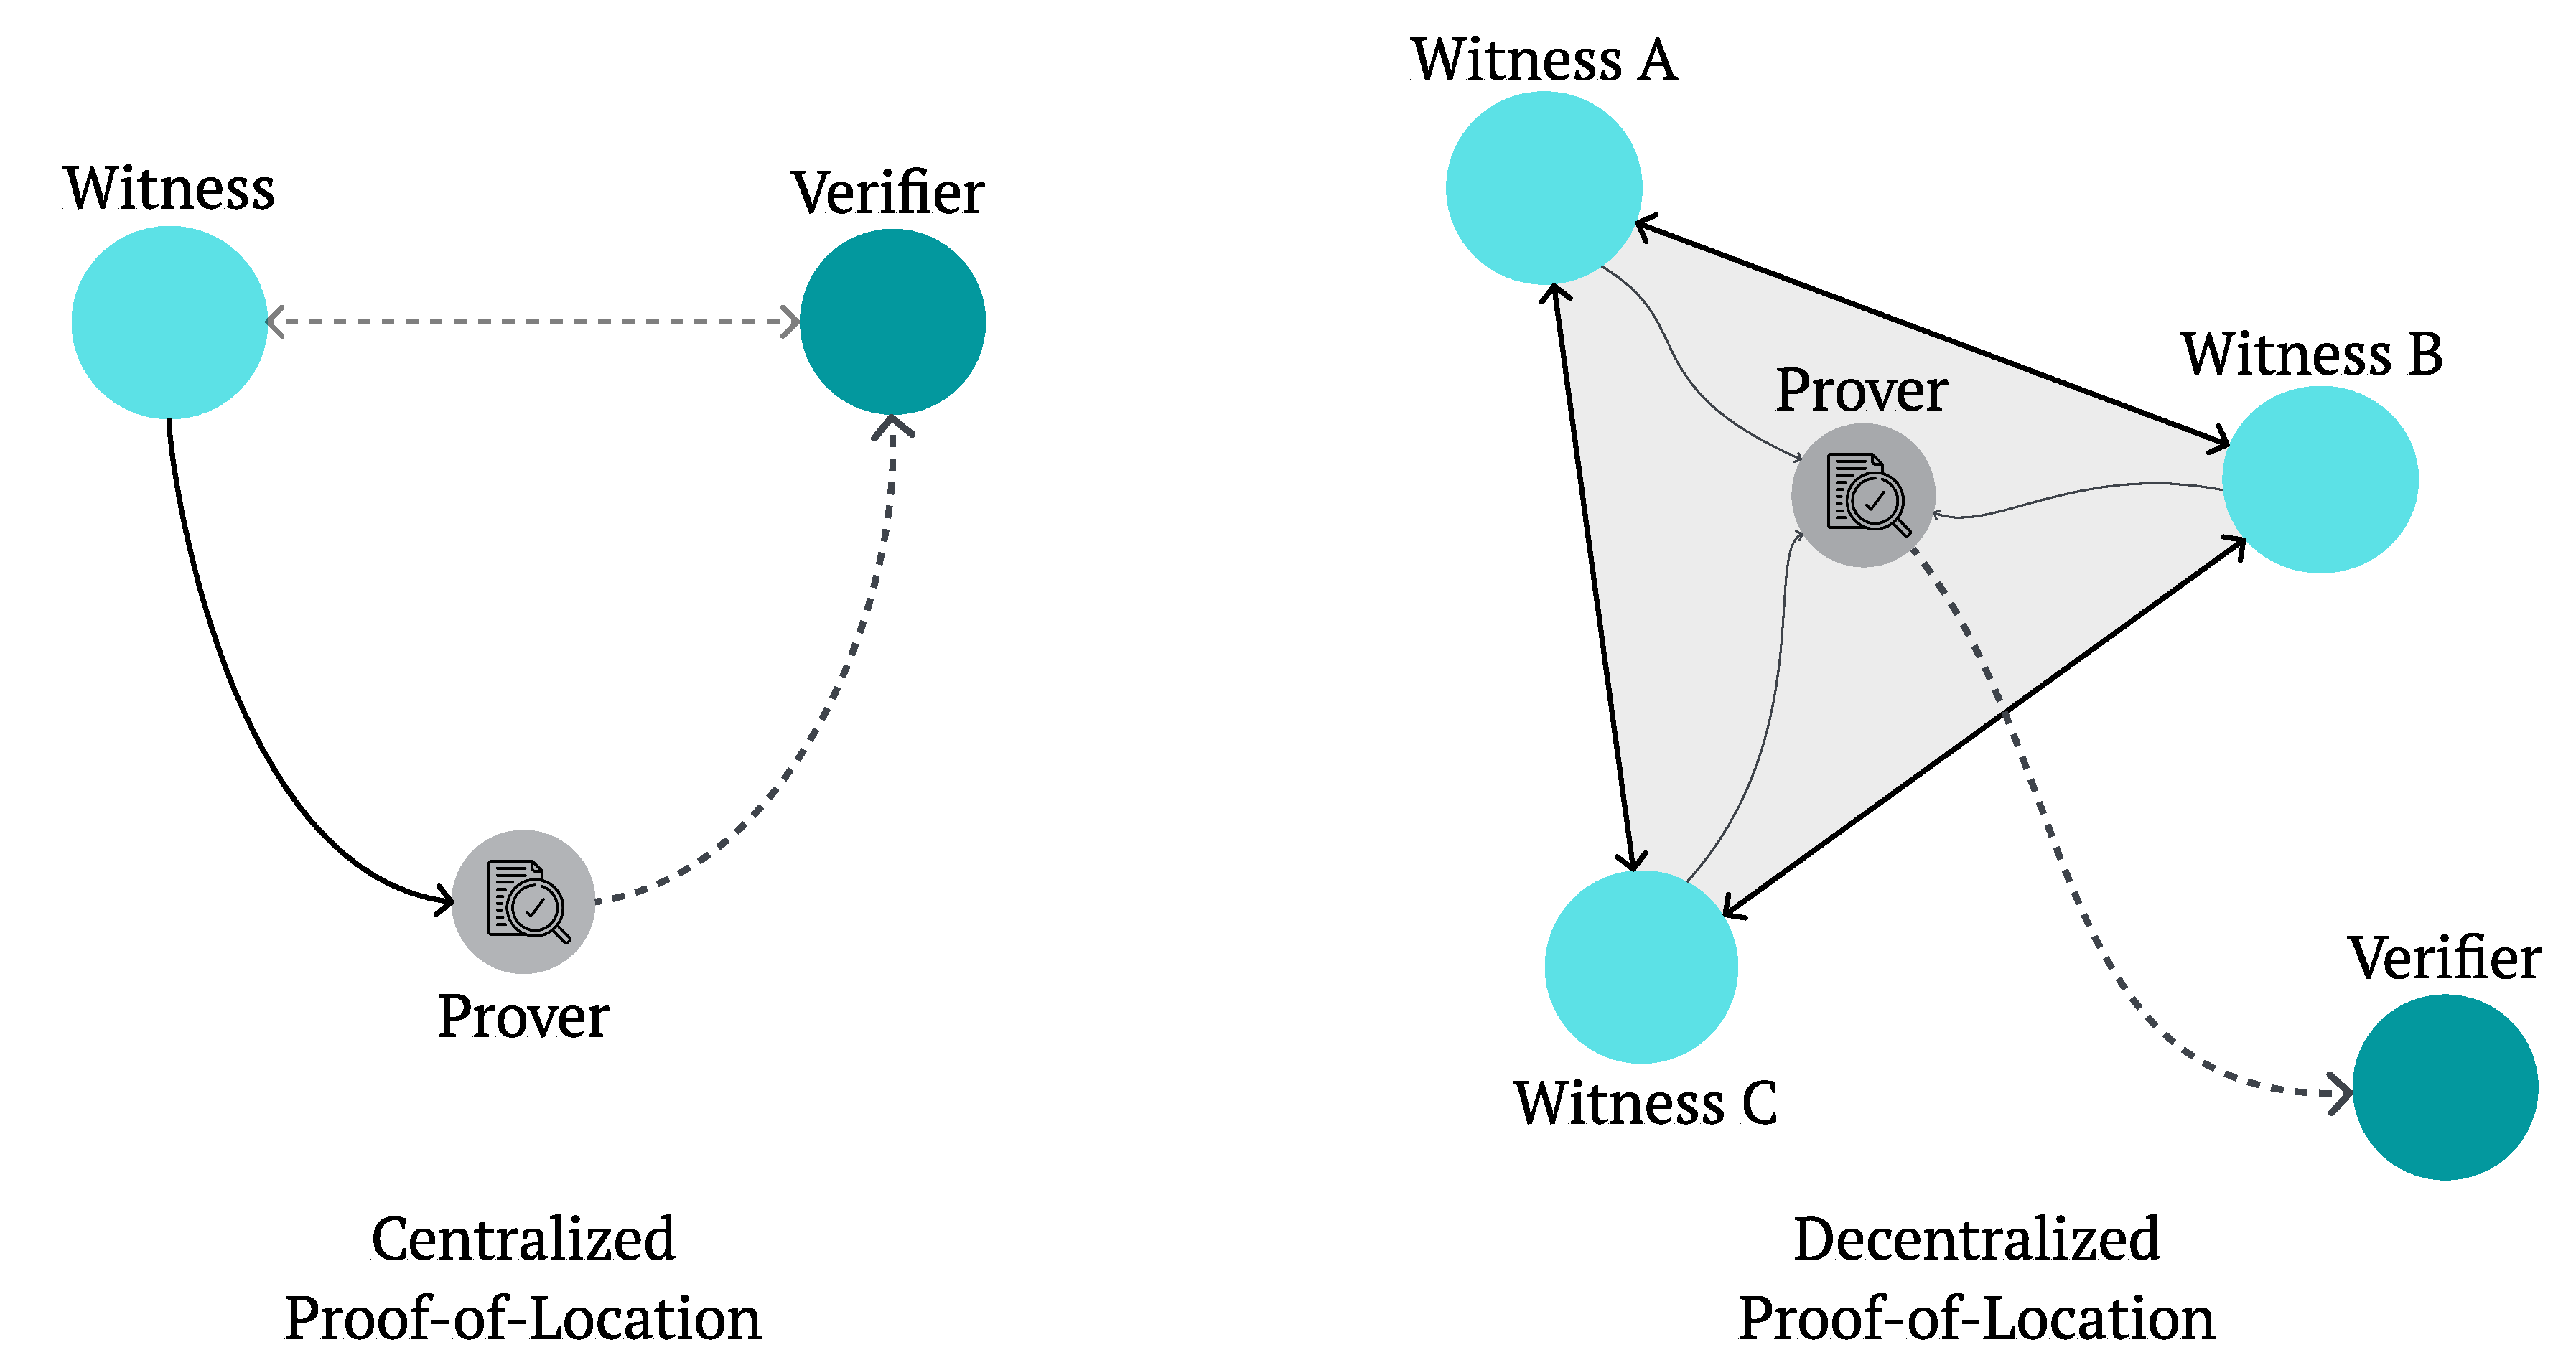
\includegraphics[width=0.9\textwidth]{proof-of-location-protocol-entities.pdf}
    \caption{The entities involved in a \pol{} protocol. The left side of the figure represents the typical arrangements of a centralized protocol, where the witness and the verifier may establish some bond between each other. The right side shows the configuration of a decentralized and trustless solution, where a quorum of witnesses attests the prover's location. Chapter~\ref{sec:related-work} will describe these possible configurations in greater detail, discriminating both their infrastructural layouts and their trust assumptions.}
    \label{fig:proof-of-location-protocol-entities}
    \end{center}
\end{figure}

\TODO{Add arrows legend to the figure: short-range and synchronously, asynchronous communitcation, etc...}

Inspired by \cite{nasrulin2018robust, dupin2018location}, we now introduce a substantially formal but general definition of the \pol{} problem, along with some of its desirable properties:

\paragraph{Definition 1 (\pol{}).} A \pol{} is a verifiable digital certificate that attests the presence of a prover $\sigma$ at location $l$ and time $t$.

\paragraph{Definition 2 (Completeness).} A \pol{} is complete if the prover $\sigma$ is attested at location $l$ and time $t$, by a set of witnesses $\omega \in W$.

\paragraph{Definition 3 (Spatio-temporal Soundness).} A \pol{} is spatio-temporally sound if it is generally hard for the prover $\sigma$ to obtain, forge, or modify a complete \pol{}, if not physically present at location $l$ and time $t$.

\paragraph{Definition 4 (Non-transferability).} A \pol{} is non-transferable if valid only for the prover $\sigma$ that obtained it.

\paragraph{Definition 5 (Correctness).} A complete \pol{}, generated by an honest prover $\sigma$, in cooperation with honest witnesses $\omega \in W$, must always be accepted by an honest verifier $\nu$.\\

Additional properties may be protocol specific, but the above definitions are generally considered to be the most common and desirable properties of a \pol{} protocol. Further formalizations can be found in the works dissected in Chapter~\ref{sec:related-work}.

\subsubsection{Common Threat Models}

Like with any technology that involves the collection and processing of sensitive and tamper-prone location data, \pol{} systems must be designed and implemented with a keen awareness of the threat landscape. The threat models of these systems are very often intricately multisided, encompassing a diverse range of actors, motives, and attack vectors. In this context, it is crucial to understand not only the technical mechanisms of \pol{} systems, but also the broader factors that shape their security and privacy risks. 

Some common scenarios that may affect the security of \pol{} systems are, for instance, malicious provers that may attempt to forge location claims, or witnesses that may attempt to collude with other entities to falsify the information. Adversary efforts may also be observed in the form of baleful provers, or witnesses, that may try to respectively impersonate other peers. Sybil attacks are too on the horizon of possible threats, often employed to disrupt the operation of the system by flooding it with fake participants \cite{nasrulin2018robust}. Other works have also considered semi-honest adversaries that, despite following the protocol rules, may try to learn additional information from the messages exchanged \cite{dupin2018location}. These and other attack vectors are further dissected in Chapter~\ref{sec:related-work}, with reference to the multiple solutions that attempt at being shielded from these malicious scenarios.

\subsubsection{Application Scenarios}
\label{sec:background-proof-of-location-application-scenarios}

The concept of verifiable and digital \pol{} has an inevitably wide range of applications, as deconstructed by Sariou and Alec, in \cite{saroiu2009enabling}. For instance, in customer reward systems, \pol{} can be used to provide incentives to customers who visit physical stores. Retailers can create loyalty programs that offer rewards to customers who visit their stores and verify their physical presence. The rewards can be tailored to individual customer preferences, based on their location data, and can encourage customer retention. In location-authenticated business review systems, \pol{} can be used to verify the authenticity of customer reviews. By requiring customers to verify their physical presence at the business location, businesses can prevent fake reviews and ensure that only genuine customer feedback is posted. In location-restricted web content delivery, \pol{} can be used to limit access to online content based on the user's physical location. For example, a video streaming service may use verifiable \pol{} to prevent users from accessing content outside legally allowed regions or countries. In voter's physical presence verification, a \pol{} protocol can be set to prevent voter fraud in multiple levels, by verifying that voters are physically present at the polling stations. This technology may consequently increase the integrity of the physical voting process and ensure that only eligible voters are allowed to vote. Additional application scenarios can be derived from the above, while many others are yet to be discovered.

Furthermore, there is work by Pournaras \cite{pournaras2020proof} that goes beyond these specific cases and theorizes about an augmented democracy approach to smart city development, using \pol{}. In this hypothesis, \pol{} is used to create a transparent and participatory decision-making process by enabling citizens to verify their physical presence at public meetings and events. This can increase civic engagement and promote democratic values by ensuring that all voices are counted and represented in the decision-making process. Given all this, digital and verifiable \pol{} has a wide range of applications that may disruptively benefit individuals, businesses, and the society as a whole. Chapter~\ref{sec:related-work}, afterwards, gives a more nuanced overview of both the evolution of the protocols and specific use cases that these multiple solutions aim at covering.